% -----------------------------*- LaTeX -*------------------------------
\documentclass[UTF8]{report}
% ------------------------------------------------------------------------
% Packages
% ------------------------------------------------------------------------
\usepackage{ctex} % 支持中文
\usepackage[body={7in, 9in},left=1in,right=1in]{geometry} % 改变页边距
\usepackage{amsmath} % AMS 的数学宏包
\usepackage{amsfonts} % AMS 的数学字体宏包
\usepackage{amssymb} % AMS 符号库
\usepackage{bm} % 数学公式中的黑斜体
\usepackage{amsthm} % AMS 的定理环境宏包
\usepackage{graphicx} % 插图
\usepackage{subfigure} % 插子图
\usepackage{nicefrac} % 好看的分数
\usepackage{mathrsfs} % mathscr font
\usepackage{caption} % caption
\usepackage{algorithm,algorithmicx} % 伪代码支持宏包
\usepackage[noend]{algpseudocode} % 伪代码
\usepackage{fancyhdr} % 设置页眉、页脚
\usepackage{adjustbox} % 图片尺寸自动调整
\usepackage{esint} % 积分符号
\usepackage{mathtools} % 数学宏包的重要补充
\usepackage{upgreek} % 数学环境的直立希腊字母
\usepackage{enumitem} % 使用enumitem宏包, 改变列表项的格式
\usepackage{color} % 支持彩色
\usepackage{extarrows} % 任意长度的箭头
\usepackage{tikz} % 绘图
\usepackage{forest} % 绘树
\usepackage{xcolor} % 颜色宏包
\usepackage{breqn} % 公式自动换行
\usepackage{fontsize} % 字体大小
\usepackage[framemethod=TikZ]{mdframed} % 给文字加框
\usepackage{fontspec} % 字体库
\usepackage{bigstrut} % 用于表格中的换行
\usepackage{multirow} % 表格中多行单元格合并
\usepackage{multicol} % 表格中多列单元格合并
\usepackage{longtable} % 长表格
\usepackage{rotating} % 旋转图形和表格      以上三者用于绘制三线表
\usepackage{booktabs} % 三线表宏包
\usepackage{scribe} % Scribe 模板
\usepackage{diagbox} % 表格斜线
\usepackage{listings} % 插入代码
\usepackage{verbatim} % 多行注释
\usepackage{ifplatform} % 检测编译平台
\usepackage{hyperref} % 超链接
\usepackage{mathrsfs} % 花体
\usepackage{pgffor} % foreach
\usepackage{circuitikz} % 画电路图
\usepackage{svg} % 插入svg
\usetikzlibrary{shapes.geometric, arrows} % 引入流程图需要的库
\usetikzlibrary{automata} % 引入automata库
\usetikzlibrary{shapes,arrows,positioning,chains} % 引入positioning库
% ------------------------------------------------------------------------
% Macros
% ------------------------------------------------------------------------
%~~~~~~~~~~~~~~~
% Utility latin
%~~~~~~~~~~~~~~~
\newcommand{\ie}{\textit{i.e.}}
\newcommand{\eg}{\textit{e.g.}}
%~~~~~~~~~~~~~~~
% Environment shortcuts
%~~~~~~~~~~~~~~~
\newcommand{\balign}[1]{\ealign{\begin{align}#1\end{align}}}
\newcommand{\baligns}[1]{\ealigns{\begin{align*}#1\end{align*}}}
\newcommand{\bitemize}[1]{\eitemize{\begin{itemize}#1\end{itemize}}}
\newcommand{\benumerate}[1]{\eenumerate{\begin{enumerate}#1\end{enumerate}}}
%~~~~~~~~~~~~~~~
% Text with quads around it
%~~~~~~~~~~~~~~~
\newcommand{\qtext}[1]{\quad\text{#1}\quad}
%~~~~~~~~~~~~~~~
% Shorthand for math formatting
%~~~~~~~~~~~~~~~
\newcommand{\mbb}[1]{\mathbb{#1}}
\newcommand{\mbi}[1]{\boldsymbol{#1}} % Bold and italic (math bold italic)
\newcommand{\mbf}[1]{\mathbf{#1}}
\newcommand{\mc}[1]{\mathcal{#1}}
\newcommand{\mrm}[1]{\mathrm{#1}}
\newcommand{\tbf}[1]{\textbf{#1}}
\newcommand{\tsc}[1]{\textsc{#1}}
%\def\\langle {{\langle }}
%\def\\rangle {{\rangle }}
\newcommand{\sT}{\sf T}
\newcommand{\grad}{\nabla}
\newcommand{\Proj}{\Pi}
%~~~~~~~~~~~~~~~
% Common sets 定义数集符号
%~~~~~~~~~~~~~~~
\newcommand{\R}{\mathbb{R}}
\newcommand{\Z}{\mathbb{Z}}
\newcommand{\Q}{\mathbb{Q}}
\newcommand{\N}{\mathbb{N}}
\newcommand{\C}{\mathbb{C}}
\newcommand{\reals}{\mathbb{R}} % Real number symbol
\newcommand{\integers}{\mathbb{Z}} % Integer symbol
\newcommand{\rationals}{\mathbb{Q}} % Rational numbers
\newcommand{\naturals}{\mathbb{N}} % Natural numbers
\newcommand{\complex}{\mathbb{C}} % Complex numbers
%~~~~~~~~~~~~~~~
% Common functions
%~~~~~~~~~~~~~~~
\renewcommand{\exp}[1]{\operatorname{exp}\left(#1\right)} % Exponential
\newcommand{\indic}[1]{\mbb{I}\left(#1\right)} % Indicator function
\newcommand{\indicsub}[2]{\mbb{I}_{#2}\left(#1\right)} % Indicator function
\newcommand{\argmax}{\mathop\mathrm{arg\, max}} % Defining math symbols
\newcommand{\argmin}{\mathop\mathrm{arg\, min}}
\renewcommand{\arccos}{\mathop\mathrm{arccos}}
\newcommand{\dom}{\mathop\mathrm{dom}} % Domain
\newcommand{\range}{\mathop\mathrm{range}} % Range
\newcommand{\diag}{\mathop\mathrm{diag}}
\newcommand{\tr}{\mathop\mathrm{tr}}
\newcommand{\abs}{\mathop\mathrm{abs}}
\newcommand{\card}{\mathop\mathrm{card}}
\newcommand{\sign}{\mathop\mathrm{sign}}
\newcommand{\prox}{\mathrm{prox}} % prox
\newcommand{\rank}[1]{\mathrm{rank}(#1)}
\newcommand{\supp}[1]{\mathrm{supp}(#1)}
\newcommand{\norm}[1]{\lVert#1\rVert}
%~~~~~~~~~~~~~~~
% Common probability symbols
%~~~~~~~~~~~~~~~
\newcommand{\family}{\mathcal{P}} % probability family / statistical model
\newcommand{\iid}{\stackrel{\mathrm{iid}}{\sim}}
\newcommand{\ind}{\stackrel{\mathrm{ind}}{\sim}}
\newcommand{\E}{\mathbb{E}} % Expectation symbol
\newcommand{\Earg}[1]{\E\left[#1\right]}
\newcommand{\Esubarg}[2]{\E_{#1}\left[#2\right]}
\renewcommand{\P}{\mathbb{P}} % Probability symbol
\newcommand{\Parg}[1]{\P\left(#1\right)}
\newcommand{\Psubarg}[2]{\P_{#1}\left[#2\right]}
%\newcommand{\Cov}{\mrm{Cov}} % Covariance symbol
%\newcommand{\Covarg}[1]{\Cov\left[#1\right]}
%\newcommand{\Covsubarg}[2]{\Cov_{#1}\left[#2\right]}
%\newcommand{\model}{\mathcal{P}} % probability family / statistical model
%~~~~~~~~~~~~~~~
% Distributions
%~~~~~~~~~~~~~~~
%\newcommand{\Gsn}{\mathcal{N}}
%\newcommand{\Ber}{\textnormal{Ber}}
%\newcommand{\Bin}{\textnormal{Bin}}
%\newcommand{\Unif}{\textnormal{Unif}}
%\newcommand{\Mult}{\textnormal{Mult}}
%\newcommand{\NegMult}{\textnormal{NegMult}}
%\newcommand{\Dir}{\textnormal{Dir}}
%\newcommand{\Bet}{\textnormal{Beta}}
%\newcommand{\Gam}{\textnormal{Gamma}}
%\newcommand{\Poi}{\textnormal{Poi}}
%\newcommand{\HypGeo}{\textnormal{HypGeo}}
%\newcommand{\GEM}{\textnormal{GEM}}
%\newcommand{\BP}{\textnormal{BP}}
%\newcommand{\DP}{\textnormal{DP}}
%\newcommand{\BeP}{\textnormal{BeP}}
%\newcommand{\Exp}{\textnormal{Exp}}
%~~~~~~~~~~~~~~~
% Theorem-like environments
%~~~~~~~~~~~~~~~
%\theoremstyle{definition}
%\newtheorem{definition}{Definition}
%\newtheorem{example}{Example}
%\newtheorem{problem}{Problem}
%\newtheorem{lemma}{Lemma}
%~~~~~~~~~~~~~~~
% 组合数学的模板和作业里用到的一些宏包和自定义命令
%~~~~~~~~~~~~~~~
\renewcommand{\emph}[1]{\begin{kaishu}#1\end{kaishu}}
\newcommand{\falfac}[1]{^{\underline{#1}}}
\newcommand{\binomfrac}[2]{\frac{#1^{\underline{#2}}}{#2!}}
\newcommand{\ceil}[1]{\left\lceil #1 \right\rceil}
\newcommand{\floor}[1]{\left\lfloor #1 \right\rfloor}
\newcommand{\suminfty}[2]{\sum_{#1=#2}^{\infty}}
\newcommand{\suminftyk}[0]{\sum_{k=0}^{\infty}}
\newcommand{\sumint}[3]{\sum_{#1=#2}^{#3}}
\newcommand{\sumintk}[2]{\sum_{k=#1}^{#2}}
\newcommand{\suminti}[2]{\sum_{i=#1}^{#2}}
%~~~~~~~~~~~~~~~
% 定义新命令
%~~~~~~~~~~~~~~~
\newcommand*{\unit}[1]{\mathop{}\!\mathrm{#1}}
\newcommand*{\dif}{\mathop{}\!\mathrm{d}}%微分算子 d
\newcommand*{\pdif}{\mathop{}\!\partial}%偏微分算子
\newcommand*{\cdif}{\mathop{}\!\nabla}%协变导数、nabla 算子
\newcommand*{\laplace}{\mathop{}\!\Delta}%laplace 算子
\newcommand*{\deri}[1]{\mathrm{d} #1}
\newcommand*{\deriv}[2]{\frac{\mathrm{d} #1}{\mathrm{d} {#2}}}
\newcommand*{\derivh}[3]{\frac{\mathrm{d}^{#1} #2}{\mathrm{d} {#3^{#1}}}}
\newcommand*{\pderiv}[2]{\frac{\partial #1}{\partial {#2}}}
\newcommand*{\pderivh}[3]{\frac{\partial^{#1} #2}{\partial {#3^{#1}}}}
\newcommand*{\dderiv}[2]{\dfrac{\mathrm{d} #1}{\mathrm{d} {#2}}}
\newcommand*{\dderivh}[3]{\dfrac{\mathrm{d}^{#1} #2}{\mathrm{d} {#3^{#1}}}}
\newcommand*{\dpderiv}[2]{\dfrac{\partial #1}{\partial {#2}}}
\newcommand*{\dpderivh}[3]{\dfrac{\partial^{#1} #2}{\partial {#3^{#1}}}}
\newcommand{\me}[1]{\mathrm{e}^{#1}}%e 指数
\newcommand{\mi}{\mathrm{i}}%虚数单位
%\newcommand{\mc}{\mathrm{c}}%光速 定义与mathcal冲突
\newcommand{\red}[1]{\textcolor{red}{#1}}
\newcommand{\blue}[1]{\textcolor{blue}{#1}}
%\newcommand{\Rome}[1]{\setcounter{rome}{#1}\Roman{rome}}
%~~~~~~~~~~~~~~~
% 公式环境中箭头符号的简写
%~~~~~~~~~~~~~~~
\newcommand{\ra}{\rightarrow}
\newcommand{\Ra}{\Rightarrow}
\newcommand{\la}{\leftarrow}
\newcommand{\La}{\Leftarrow}
\newcommand{\lra}{\leftrightarrow}
\newcommand{\Lra}{\Leftrightarrow}
\newcommand{\lgla}{\longleftarrow}
\newcommand{\Lgla}{\Longleftarrow}
\newcommand{\lgra}{\longrightarrow}
\newcommand{\Lgra}{\Longrightarrow}
\newcommand{\lglra}{\longleftrightarrow}
\newcommand{\Lglra}{\Longleftrightarrow}
%~~~~~~~~~~~~~~~
% 一些数学的环境设置
%~~~~~~~~~~~~~~~
%\newcounter{counter_exm}\setcounter{counter_exm}{1}
%\newcounter{counter_prb}\setcounter{counter_prb}{1}
%\newcounter{counter_thm}\setcounter{counter_thm}{1}
%\newcounter{counter_lma}\setcounter{counter_lma}{1}
%\newcounter{counter_dft}\setcounter{counter_dft}{1}
%\newcounter{counter_clm}\setcounter{counter_clm}{1}
%\newcounter{counter_cly}\setcounter{counter_cly}{1}
\newtheorem{theorem}{{\hskip 1.7em \bf 定理}}
\newtheorem{lemma}[theorem]{\hskip 1.7em 引理}
\newtheorem{proposition}[theorem]{\hskip 1.7em 命题}
\newtheorem{claim}[theorem]{\hskip 1.7em 断言}
\newtheorem{corollary}[theorem]{\hskip 1.7em 推论}
% \newcommand{\problem}[1]{{\setlength{\parskip}{10pt}\noindent \bf{#1}}}
\newenvironment{solution}{{\noindent \bf 解 \quad}}{}
\newenvironment{remark}{{\noindent \bf 注 \quad}}{}
\newenvironment{definition}{{\noindent \bf 定义 \quad}}{}
\renewenvironment{proof}{{\setlength{\parskip}{7pt}\noindent\hskip 2em \bf 证明 \quad}}{\hfill$\qed$\par}
\newenvironment{example}{{\noindent\bf 例 \quad}}{\hfill$\qed$\par}
%\newenvironment{concept}[1]{{\bf #1\quad} \begin{kaishu}} {\end{kaishu}\par}
%~~~~~~~~~~~~~~~
% 本.tex文档中特殊定义命令
%~~~~~~~~~~~~~~~
\newcommand{\lno}[1]{\overline{#1}}
\newcommand{\NP}{\mathrm{NP}}
\newcommand{\coNP}{\mathrm{coNP}}
% \newcommand{\ISO}{\mathrm{ISO}}
\newcommand{\SAT}{\mathrm{SAT}}
\newcommand{\USAT}{\mathrm{USAT}}
% \newcommand{\threeSAT}{\mathrm{3\text{-}SAT}}
\renewcommand{\P}{\mathrm{P}}
% \mathchardef\mhyphen="2D
% \newcommand{\CNF}{\mathrm{CNF}}
% \newcommand{\DNF}{\mathrm{DNF}}
% \newcommand{\SetSp}{\mathrm{SET\text{-}SPLITTING}}
% \newcommand{\PUZZLE}{\mathrm{PUZZLE}}
% \newcommand{\SPATH}{\mathrm{SPATH}}
% \newcommand{\LPATH}{\mathrm{LPATH}}
% \newcommand{\UHAMPATH}{\mathrm{UHAMPATH}}
\newcommand{\SPACE}{\mathrm{SPACE}}
\newcommand{\NSPACE}{\mathrm{NSPACE}}
\newcommand{\PSPACE}{\mathrm{PSPACE}}
\newcommand{\NPSPACE}{\mathrm{NPSPACE}}
\newcommand{\DFA}{\mathrm{DFA}}
\newcommand{\NFA}{\mathrm{NFA}}
\newcommand{\TQBF}{\mathrm{TQBF}}
% \newcommand{\L}{\mathrm{L}}
\renewcommand{\O}{\mathrm{O}}
\newcommand{\NL}{\mathrm{NL}}
\newcommand{\coNL}{\mathrm{coNL}}
\newcommand{\LADDER}{\mathrm{LADDER_{DFA}}}
\newcommand{\hd}{\mathrm{\text{-}hard}}
\newcommand{\ADD}{\mathrm{ADD}}
\newcommand{\STCN}{\mathrm{STRONGLY\text{-}CONNECTED}}
\newcommand{\PATH}{\mathrm{PATH}}
\newcommand{\A}{\mathrm{A}}
%使用align环境公式换页
\allowdisplaybreaks[4]

\definecolor{dkgreen}{rgb}{0,0.6,0}
\definecolor{gray}{rgb}{0.5,0.5,0.5}
\definecolor{mauve}{rgb}{0.58,0,0.82}
\lstset{
  frame=tb,
  aboveskip=3mm,
  belowskip=3mm,
  showstringspaces=false,
  columns=flexible,
  framerule=1pt,
  rulecolor=\color{gray!35},
  backgroundcolor=\color{gray!5},
  basicstyle={\small\ttfamily},
  numbers=left,
  numberstyle=\ttfamily\color{gray},
  keywordstyle=\color{blue},
  commentstyle=\color{dkgreen},
  stringstyle=\color{mauve},
  breaklines=true,
  breakatwhitespace=true,
  tabsize=3,
}

\lstdefinelanguage{LoongArch}{
  morekeywords={la, lw, addi, sw, li, syscall, beqz, add, move, bge, blt, b, sub, ret, beq, bne},  
  literate={ll.w}{{{\color{blue}ll.w}}}1
           {sc.w}{{{\color{blue}sc.w}}}1
           {addi.d}{{{\color{blue}addi.d}}}1
           {st.d}{{{\color{blue}st.d}}}1
           {st.w}{{{\color{blue}st.w}}}1
           {ldptr.w}{{{\color{blue}ldptr.w}}}1
           {slli.d}{{{\color{blue}slli.d}}}1
           {ld.d}{{{\color{blue}ld.d}}}1
           {stptr.w}{{{\color{blue}stptr.w}}}1
           {slli.w}{{{\color{blue}slli.w}}}1
           {ld.w}{{{\color{blue}ld.w}}}1
           {addi.w}{{{\color{blue}addi.w}}}1
           {add.d}{{{\color{blue}add.d}}}1
           {sub.w}{{{\color{blue}sub.w}}}1
           {li.w}{{{\color{blue}li.w}}}1
           {bstrpick.d}{{{\color{blue}bstrpick.d}}}1
           {alsl.d}{{{\color{blue}alsl.d}}}1,
  morecomment=[l]{\#},
  frame=tb,
  aboveskip=3mm,
  belowskip=3mm,
  showstringspaces=false,
  columns=flexible,
  framerule=1pt,
  rulecolor=\color{gray!35},
  backgroundcolor=\color{gray!5},
  basicstyle={\small\ttfamily},
  numbers=left,
  numberstyle=\ttfamily\color{gray},
  keywordstyle=\color{blue},
  commentstyle=\color{dkgreen},
  stringstyle=\color{mauve},
  breaklines=true,
  breakatwhitespace=true,
  tabsize=3,
}

% 设置超链接样式
\hypersetup{
    colorlinks=true,       % 将链接颜色设置为 true
    linkcolor=magenta,        % 内部链接颜色
    filecolor=magenta,     % 文件链接颜色
    urlcolor=blue,         % URL 链接颜色
    citecolor=green,       % 引用链接颜色
}

\tikzstyle{startstop} = [rectangle, rounded corners, minimum width=3cm, minimum height=1cm,text centered, draw=black, fill=red!30]
\tikzstyle{process} = [rectangle, minimum width=3cm, minimum height=1cm, text centered, draw=black, fill=orange!30]
\tikzstyle{decision} = [diamond, minimum width=3cm, minimum height=1cm, text centered, draw=black, fill=green!30]
\tikzstyle{arrow} = [thick,->,>=stealth]

\ifwindows
    \setmainfont{Times New Roman}
    \setsansfont{Times New Roman}
    \setmonofont{Consolas}
    \setCJKmainfont{SimHei}
    \setCJKsansfont{SimSun}
    \setCJKmonofont{FangSong}
\fi

\ifmacosx
    \setmainfont{Times New Roman}
    \setsansfont{Times New Roman}
    \setmonofont{Menlo}
    \setCJKmainfont{Heiti SC}
    \setCJKsansfont{STSong}
    \setCJKmonofont{STFangsong}
\fi

\punctstyle{kaiming}

\begin{document}

\pagestyle{fancy}

\reporttype{Homework}                 % required
\course{Computer Architecture} 				% optional
\coursetitle{System Evaluation \& Performance Analysis}	    % optional
\semester{Fall 2024}			    % optional
\lecturer{Hu Weiwu}			% optional
\scribe{2022K8009929010 Zhang Jiawei}			% required
\lecturenumber{12}				% required (must be a number)
\lecturedate{December 12}			% required (omit year)
\maketitle

\noindent
\textbf{12.1}

所写测试最大MIPS的程序如下:

\begin{lstlisting}[language=C]
    #include <stdio.h>
    #include <time.h>
    
    int main() {
        long long instructions = 0; // 指令计数
        int a = 0;
        clock_t start, end;
    
        // 开始计时
        start = clock();
    
        // 执行整数加法指令
        while (instructions < 1e9) { // 1 billion iterations
            a += 1;
            instructions++;
        }
    
        // 结束计时
        end = clock();
    
        // 计算时间(秒)
        double elapsed_time = (double)(end - start) / CLOCKS_PER_SEC;
    
        // 计算 MIPS
        double mips = (instructions / 1e6) / elapsed_time;
    
        printf("Elapsed time: %.2f seconds\n", elapsed_time);
        printf("MIPS: %.2f\n", mips);
    
        return 0;
    }
\end{lstlisting}

运行结果如下图所示:

\begin{figure}[H]
    \centering
    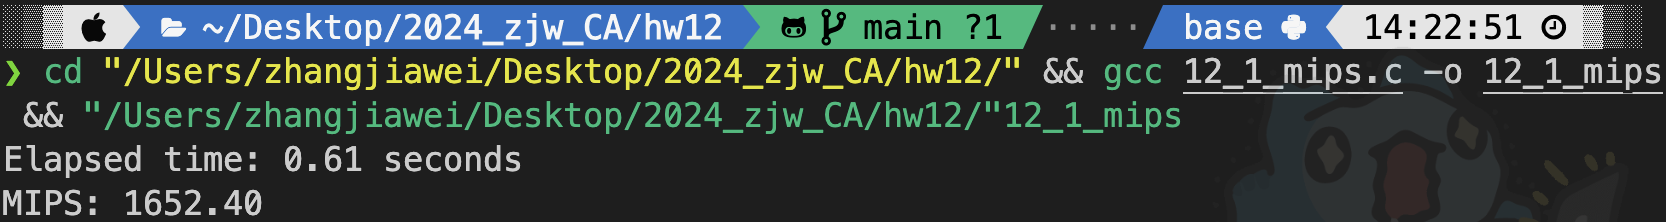
\includegraphics[width=0.8\textwidth]{img/maxMIPS.png}
    \caption{最大MIPS}
\end{figure}

所写测试最大MFLOPS的程序如下:

\begin{lstlisting}[language=C]
    #include <stdio.h>
    #include <time.h>
    
    int main() {
        long long operations = 0; // 浮点操作计数
        double x = 1.0, y = 2.0, z;
        clock_t start, end;
    
        // 开始计时
        start = clock();
    
        // 执行浮点运算(乘法)
        while (operations < 1e9) { // 1 billion iterations
            z = x * y;
            operations++;
        }
    
        // 结束计时
        end = clock();
    
        // 计算时间(秒)
        double elapsed_time = (double)(end - start) / CLOCKS_PER_SEC;
    
        // 计算 MFLOPS
        double mflops = (operations / 1e6) / elapsed_time;
    
        printf("Elapsed time: %.2f seconds\n", elapsed_time);
        printf("MFLOPS: %.2f\n", mflops);
    
        return 0;
    }
\end{lstlisting}

运行结果如下图所示:

\begin{figure}[H]
    \centering
    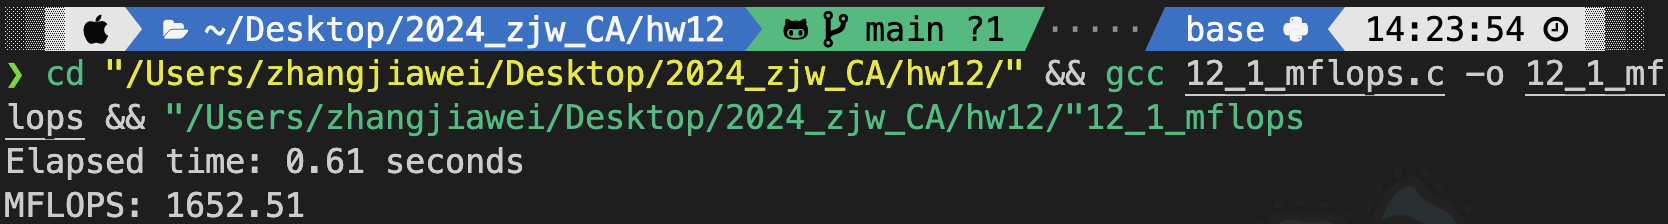
\includegraphics[width=0.8\textwidth]{img/maxMFLOPS.png}
    \caption{最大MFLOPS}
\end{figure}

\noindent
\textbf{12.2}

\begin{enumerate}[label=(\arabic*)]
    \item STREAM v1 过于古老,没有找到源码,故使用 STREAM v5.10 版本。测试结果如下:
    
    \begin{lstlisting}
        -------------------------------------------------------------
        STREAM version $Revision: 5.10 $
        -------------------------------------------------------------
        This system uses 8 bytes per array element.
        -------------------------------------------------------------
        Array size = 10000000 (elements), Offset = 0 (elements)
        Memory per array = 76.3 MiB (= 0.1 GiB).
        Total memory required = 228.9 MiB (= 0.2 GiB).
        Each kernel will be executed 10 times.
         The *best* time for each kernel (excluding the first iteration)
         will be used to compute the reported bandwidth.
        -------------------------------------------------------------
        Number of Threads requested = 8
        Number of Threads counted = 8
        -------------------------------------------------------------
        Your clock granularity/precision appears to be 1 microseconds.
        Each test below will take on the order of 5064 microseconds.
           (= 5064 clock ticks)
        Increase the size of the arrays if this shows that
        you are not getting at least 20 clock ticks per test.
        -------------------------------------------------------------
        WARNING -- The above is only a rough guideline.
        For best results, please be sure you know the
        precision of your system timer.
        -------------------------------------------------------------
        Function    Best Rate MB/s  Avg time     Min time     Max time
        Copy:           76477.3     0.002154     0.002092     0.002254
        Scale:          59498.9     0.002765     0.002689     0.002859
        Add:            59850.9     0.004163     0.004010     0.004423
        Triad:          60090.3     0.004168     0.003994     0.004465
        -------------------------------------------------------------
        Solution Validates: avg error less than 1.000000e-13 on all three arrays
        -------------------------------------------------------------
    \end{lstlisting}

    对结果进行分析,得出结论:

    \begin{itemize}
        \item Copy:
        \begin{itemize}
            \item 最佳速率:76477.3 MB/s
            \item 最小时间:0.002092 s
            \item 最大时间:0.002254 s
            \item 分析:Copy 操作的最佳速率非常高,表明内存带宽性能良好。最小时间和最大时间之间的差异较小,表明测试结果稳定。
        \end{itemize}
        \item Scale:
        \begin{itemize}
            \item 最佳速率:59498.9 MB/s
            \item 最小时间:0.002689 s
            \item 最大时间:0.002859 s
            \item 分析:Scale 操作的速率略低于 Copy 操作,但仍然表现出色。时间的波动较小,表明测试结果稳定。
        \end{itemize}
        \item Add:
        \begin{itemize}
            \item 最佳速率:59850.9 MB/s
            \item 最小时间:0.004010 s
            \item 最大时间:0.004423 s
            \item 分析:Add 操作的速率与 Scale 操作相近,表明系统在处理多数组操作时性能良好。时间的波动较小,表明测试结果稳定。
        \end{itemize}
        \item Triad:
        \begin{itemize}
            \item 最佳速率:60090.3 MB/s
            \item 最小时间:0.003994 s
            \item 最大时间:0.004465 s
            \item 分析:Triad 操作的速率与 Add 操作相近,表明系统在处理复杂内存操作时性能良好。时间的波动较小,表明测试结果稳定。
        \end{itemize}
        \item 解决方案验证通过,所有三个数组的平均误差小于 1.000000e-13,表明计算结果准确。
    \end{itemize}

    \item 由于MacBook不直接提供调节处理器频率的功能,故无法测试。但可以预计的结果是,处理器频率越高,内存带宽性能越好,但是并不会一直增加,因为内存带宽性能受到内存控制器的限制,当处理器频率过高时,内存控制器可能成为性能瓶颈,导致内存带宽性能不再提升。
    
    \item 将测试类型由 double 改为 float ,测试结果如下:
    
    \begin{lstlisting}
        -------------------------------------------------------------
        STREAM version $Revision: 5.10 $
        -------------------------------------------------------------
        This system uses 4 bytes per array element.
        -------------------------------------------------------------
        Array size = 10000000 (elements), Offset = 0 (elements)
        Memory per array = 38.1 MiB (= 0.0 GiB).
        Total memory required = 114.4 MiB (= 0.1 GiB).
        Each kernel will be executed 10 times.
         The *best* time for each kernel (excluding the first iteration)
         will be used to compute the reported bandwidth.
        -------------------------------------------------------------
        Number of Threads requested = 8
        Number of Threads counted = 8
        -------------------------------------------------------------
        Your clock granularity/precision appears to be 1 microseconds.
        Each test below will take on the order of 2130 microseconds.
           (= 2130 clock ticks)
        Increase the size of the arrays if this shows that
        you are not getting at least 20 clock ticks per test.
        -------------------------------------------------------------
        WARNING -- The above is only a rough guideline.
        For best results, please be sure you know the
        precision of your system timer.
        -------------------------------------------------------------
        Function    Best Rate MB/s  Avg time     Min time     Max time
        Copy:           78581.8     0.001097     0.001018     0.001569
        Scale:          61353.9     0.001522     0.001304     0.001815
        Add:            58826.1     0.002165     0.002040     0.002272
        Triad:          59402.4     0.002142     0.002020     0.002315
        -------------------------------------------------------------
        Solution Validates: avg error less than 1.000000e-06 on all three arrays
        -------------------------------------------------------------
    \end{lstlisting}

    与之前的结果进行对比,可以看出,float 类型的测试结果与 double 类型的测试结果相近,但是 float 类型的速率略高于 double 类型,这是因为 float 类型的数据占用内存更少,更容易被缓存,从而提高了内存带宽性能。
\end{enumerate}

\noindent
\textbf{12.3}

462.libquantum 对处理器的主要压力集中在以下几个方面:整数运算单元(ALU)的利用率、缓存命中率低导致的内存子系统压力、分支预测失败的影响、内存带宽瓶颈。

Intel ICC 能显著提升 462.libquantum 的分值,最高可达 GCC 的 2 倍以上;GCC 和 Clang 在优化复杂程序时较保守,导致 462.libquantum 的分值较低。icc 可能通过优化内存访问、提高指令并行性和改进分支效率等方式提升 462.libquantum 的性能。

\noindent
\textbf{12.4}

确实使用了 perf 测量,但是虚拟机不支持许多参数(摊手\includesvg[width=1em]{img/emoji_u1f937.svg}),故无法获得详细的 perf 测量结果。

\begin{figure}[H]
    \centering
    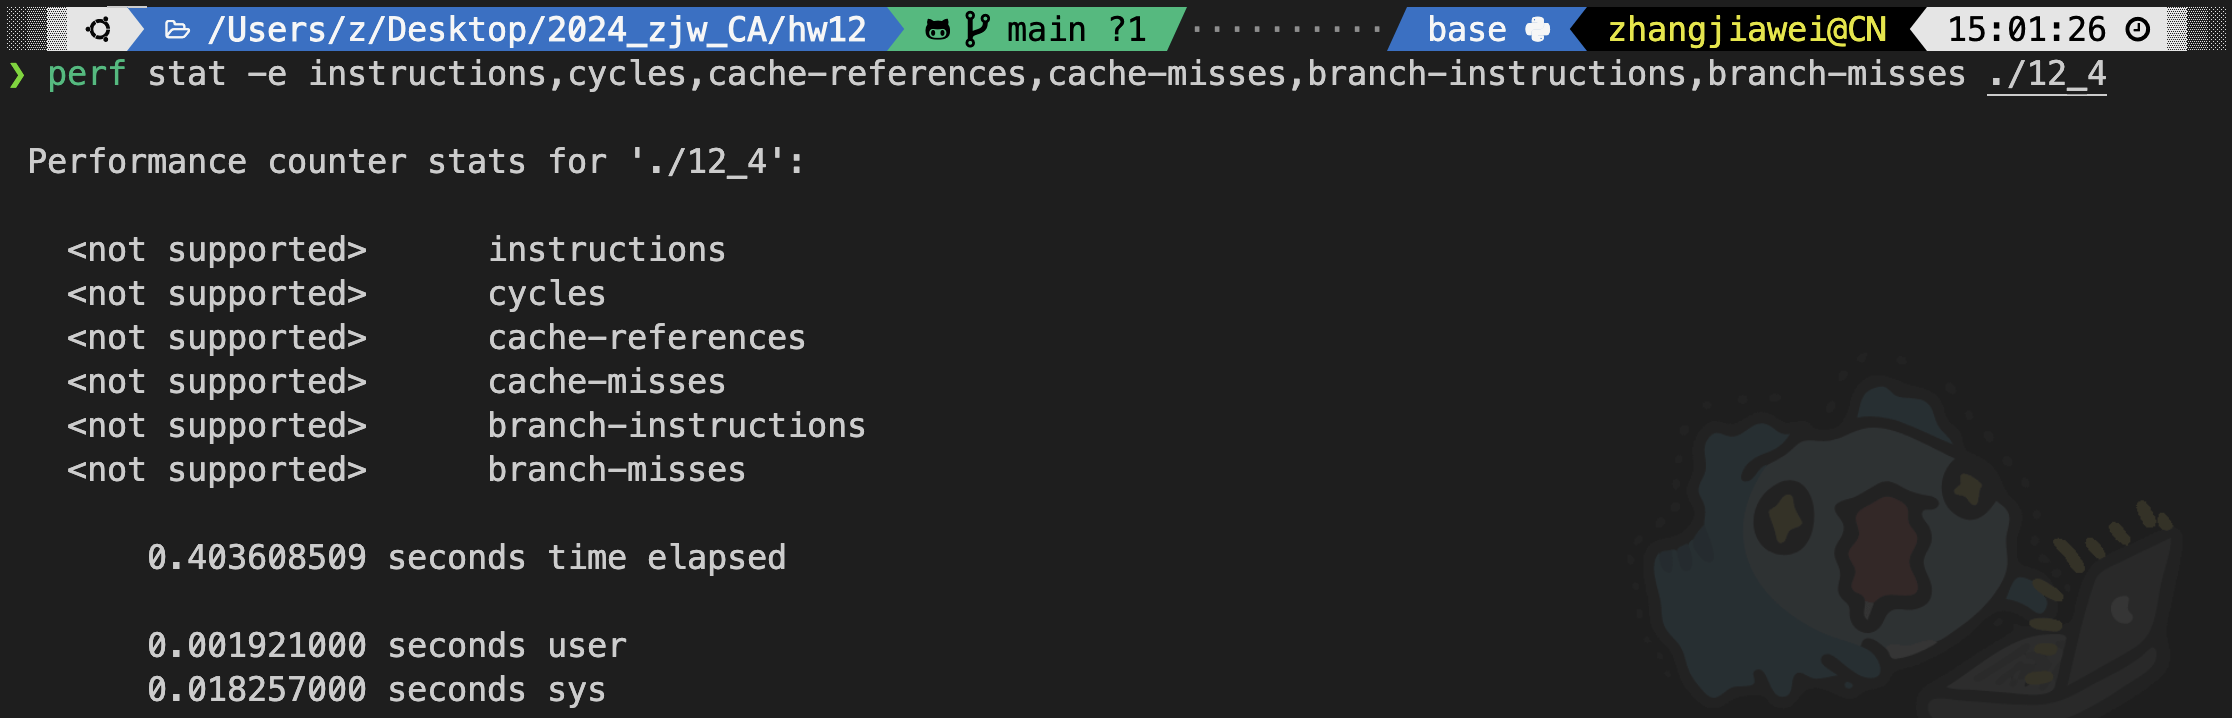
\includegraphics[width=0.8\textwidth]{img/perf.png}
    \caption{perf 测量}
\end{figure}

\noindent
\textbf{12.5}

使用gprof获得的结果如下:

\begin{lstlisting}
    %   cumulative   self              self     total           
    time   seconds   seconds    calls   s/call   s/call  name    
    99.48      3.86     3.86        1     3.86     3.86  dgefa
     0.26      3.87     0.01        1     0.01     0.01  dgesl
     0.26      3.88     0.01        1     0.01     0.01  matgen   
\end{lstlisting}

显然热点函数是 dgefa,占用了 99.48\% 的时间。

\noindent
\textbf{12.6}

测试结果如下:

\begin{lstlisting}
    stride=256
    0.00049 0.304
    0.00098 0.321
    0.00195 0.872
    0.00293 0.878
    0.00391 0.873
    0.00586 0.890
    0.00781 0.871
    0.01172 0.874
    0.01562 0.871
    0.02344 0.881
    0.03125 0.880
    0.04688 0.878
    0.06250 0.885
    0.09375 0.945
    0.12500 0.882
    0.18750 2.106
    0.25000 2.088
    0.37500 2.089
    0.50000 2.096
    0.75000 2.083
    1.00000 2.079
    1.50000 2.085
    2.00000 2.087
    3.00000 2.093
    4.00000 2.093
    6.00000 2.049
    8.00000 2.193
    12.00000 2.784
    16.00000 4.540
    24.00000 10.517
    32.00000 13.153
    48.00000 14.949
    64.00000 15.961
    96.00000 16.040
    128.00000 16.234
\end{lstlisting}

L1 缓存数据块大小在 0.49KB 到 125KB 的范围,延迟为 0.3~0.9 纳秒;

L2 缓存数据块大小在 187KB 到 1.5MB,延迟约为 2.1 纳秒;

L3 缓存数据块大小在 2MB 到 8MB,延迟约为 2.1~2.8 纳秒;

主内存数据块大小超过 16MB 后,延迟显著增加,达到 4.5 纳秒及以上。

\noindent
\textbf{12.7}

simplesim已安装成功,但alpha语言的二进制文件无法获取(摊手\includesvg[width=1em]{img/emoji_u1f937.svg})。

结果如下:

\begin{lstlisting}
    sim-outorder: SimpleScalar/Alpha Tool Set version 3.0 of March, 2023.
    Copyright (c) 1994-2003 by Todd M. Austin, Ph.D. and SimpleScalar, LLC.
    All Rights Reserved. This version of SimpleScalar is licensed for academic
    non-commercial use.  No portion of this work may be used by any commercial
    entity, or for any commercial purpose, without the prior written permission
    of SimpleScalar, LLC (info@simplescalar.com).
    
    fatal: bad magic number in executable `../spec2000-all/benchspec/CINT2000/164.gzip/run/00000001/gzip' (not an executable)    
\end{lstlisting}

\noindent
\textbf{12.8}

\begin{enumerate}
    \item 目标设备和应用场景
    \begin{itemize}
        \item \textbf{嵌入式基准测试(EEMBC)}:
        \begin{itemize}
            \item \textbf{目标设备}:嵌入式处理器、微控制器(MCU)、SoC 等。
            \item \textbf{应用场景}:实时性、低功耗、小内存占用。
            \item \textbf{测试内容}:压缩/解压缩、图像处理、信号处理、嵌入式控制等。
        \end{itemize}
        \item \textbf{桌面基准测试}:
        \begin{itemize}
            \item \textbf{目标设备}:桌面 PC、工作站、高性能服务器。
            \item \textbf{应用场景}:通用计算任务,如办公、游戏、创意设计等。
            \item \textbf{测试内容}:CPU 性能、GPU 渲染、存储性能等。
        \end{itemize}
    \end{itemize}
    
    \item 计算行为差异
    \begin{itemize}
        \item \textbf{计算复杂度}:
        \begin{itemize}
            \item 嵌入式测试:轻量化负载,数据集较小。
            \item 桌面测试:复杂负载,数据集较大。
        \end{itemize}
        \item \textbf{实时性}:
        \begin{itemize}
            \item 嵌入式测试:强调确定性和实时性。
            \item 桌面测试:关注平均性能而非实时性。
        \end{itemize}
    \end{itemize}

    \item 电源与能效
    \begin{itemize}
        \item 嵌入式测试:关注每瓦性能,强调功耗优化。
        \item 桌面测试:以峰值性能为主,能效优先级较低。
    \end{itemize}

    \item 软件架构和编译优化
    \begin{itemize}
        \item 嵌入式测试:针对特定硬件优化,轻量级 RTOS 或裸机环境。
        \item 桌面测试:运行在通用操作系统上,支持多核、多线程优化。
    \end{itemize}
\end{enumerate}

\noindent
\textbf{12.9}

\begin{itemize}
    \item \textbf{指令相关事件}
    \begin{itemize}
        \item \textbf{CPU Cycles (`cpu\_cycles`)}: 处理器核心的时钟周期总数,无论是否执行了指令。用于衡量程序执行所需的总时间。
        \item \textbf{Instructions Retired (`inst\_retired`)}: 已完成并提交的指令总数,用于评估程序的指令吞吐率。
    \end{itemize}

    \item \textbf{缓存相关事件}
    \begin{itemize}
        \item \textbf{L1 Data Cache Access (`l1d\_cache`)}: L1 数据缓存的访问次数,包括命中和未命中。
        \item \textbf{L1 Data Cache Refills (`l1d\_cache\_refill`)}: L1 数据缓存未命中后从更高级缓存或内存中加载数据的次数,反映缓存效率。
        \item \textbf{L2 Cache Access (`l2d\_cache`)}: L2 缓存的访问次数,包括数据读取和写入操作。
        \item \textbf{L2 Cache Refills (`l2d\_cache\_refill`)}: L2 缓存未命中后从主内存中加载数据的次数,表示 L2 性能和主内存压力。
    \end{itemize}

    \item \textbf{分支相关事件}
    \begin{itemize}
        \item \textbf{Branch Instructions Executed (`br\_inst\_executed`)}: 执行的分支指令总数,包括条件和无条件分支,用于分析程序的控制流。
        \item \textbf{Branch Mispredictions (`br\_mis\_pred`)}: 分支预测失败的次数,反映分支预测器的准确性。
    \end{itemize}

    \item \textbf{存储与总线相关事件}
    \begin{itemize}
        \item \textbf{Memory Accesses (`mem\_access`)}: 内存系统的总访问次数,包括指令和数据访问。
        \item \textbf{TLB Misses (`tlb\_miss`)}: 虚拟地址转换时的 TLB(翻译后备缓冲)未命中次数,反映虚拟内存管理的效率。
    \end{itemize}
\end{itemize}

\noindent
\textbf{12.10}

\begin{itemize}
    \item \textbf{提前预测性能}
    \begin{itemize}
        \item 模拟建模可以在开发阶段就预测系统性能,而性能测量需要真实系统的实现。
        \item 通过建模分析潜在的性能瓶颈,帮助设计优化。
    \end{itemize}

    \item \textbf{更低的成本和风险}
    \begin{itemize}
        \item 模拟建模不依赖昂贵的硬件设备或复杂测试环境,从而降低成本。
        \item 模拟不会对关键任务或生产环境造成影响,而性能测量可能会有风险。
    \end{itemize}

    \item \textbf{更灵活的场景测试}
    \begin{itemize}
        \item 模拟建模可以调整模型参数,测试极端或无法实现的场景。
        \item 性能测量只能反映当前环境的表现,灵活性较低。
    \end{itemize}

    \item \textbf{可扩展性强}
    \begin{itemize}
        \item 模拟建模能够分析非常复杂的系统,而性能测量往往受硬件限制。
        \item 对于大规模分布式系统或未来架构,模拟是必要的工具。
    \end{itemize}

    \item \textbf{更容易分析特定组件}
    \begin{itemize}
        \item 模拟建模可以单独分析和优化系统的某个组件。
        \item 性能测量通常关注整体表现,很难隔离某个模块进行单独分析。
    \end{itemize}

    \item \textbf{数据的全面性}
    \begin{itemize}
        \item 模拟建模能够输出细粒度数据,如时延分布和资源利用率。
        \item 性能测量的监控能力受到实际环境的限制。
    \end{itemize}
\end{itemize}

\noindent
\textbf{12.11}

\begin{itemize}
    \item \textbf{基本原理}:
    \begin{itemize}
        \item \textbf{程序行为聚类}:SimPoint 使用聚类算法(如 $k$-means),通过分析程序的基本块(basic blocks)执行频率,识别具有相似行为的程序片段(phase)。
        \item \textbf{代表性片段选择}:从程序的多个行为阶段中选择少数代表性片段进行模拟,这些片段可以很好地代表整个程序的运行特性。
        \item \textbf{加权评估}:通过对代表性片段加权,推导出全程序的性能指标,避免对所有片段进行全面模拟。
    \end{itemize}

    \item \textbf{减少模拟建模时间的原因}:
    \begin{itemize}
        \item \textbf{减少仿真长度}:SimPoint 仅模拟代表性片段,而非整个程序,从而显著减少模拟时间。
        \item \textbf{高效的阶段识别}:通过聚类算法快速定位程序的行为阶段,无需逐周期模拟程序。
        \item \textbf{适用于复杂程序}:适用于运行时间较长、行为多样的程序,避免了全程序仿真的高开销。
        \item \textbf{精度与效率的平衡}:由于代表性片段能够准确反映程序行为,SimPoint 在显著降低模拟时间的同时,保持较高的性能预测精度。
    \end{itemize}
\end{itemize}

\noindent
\textbf{12.12}

\begin{itemize}
    \item \textbf{模拟器与真实机器校准的方法}:
    \begin{itemize}
        \item \textbf{性能特征对比}:
        比较模拟器和真实机器在执行相同程序时的关键性能特征,例如指令吞吐量、分支预测命中率、缓存命中率等。
        \item \textbf{时间行为校准}:
        使用基准测试工具(如 SPEC 或 PARSEC),测量模拟器和真实机器在相同工作负载下的执行时间,调整模拟器的模型参数以匹配真实硬件的时间行为。
        \item \textbf{事件统计校准}:
        通过硬件性能监控单元(PMU)采集真实机器的微架构事件(如缓存访问、分支预测、内存延迟等),将这些数据与模拟器生成的数据进行比较和校准。
        \item \textbf{循环精确模拟}:
        针对时间敏感的应用程序,模拟器需要实现周期级别的精确模拟,与真实机器运行每个周期的行为进行对比校准。
        \item \textbf{参数调优}:
        使用自动化工具(如遗传算法或机器学习),根据真实机器的性能数据调整模拟器的参数,使模拟结果逐步逼近真实值。
    \end{itemize}

    \item \textbf{校准的评价指标}:
    \begin{itemize}
        \item \textbf{执行时间误差}:
        模拟器预测的程序执行时间与真实机器测量值之间的误差,通常以百分比表示。
        \item \textbf{性能事件误差}:
        模拟器生成的微架构事件计数(如缓存命中数、分支预测命中数)与真实机器的计数之间的差异。
        \item \textbf{指令级精确性}:
        模拟器生成的每条指令的执行行为是否与真实机器一致。
        \item \textbf{吞吐率差异}:
        模拟器预测的指令吞吐量(IPC)与真实机器的差异。
        \item \textbf{周期误差分布}:
        模拟器在每个周期上预测的性能与真实机器的误差分布,用于评估时间行为的细节一致性。
        \item \textbf{负载敏感性}:
        校准模拟器在不同工作负载下的精确性,确保其能准确预测各种场景的性能。
        \item \textbf{能耗偏差}:
        如果模拟器支持能耗估算,则需要将其与真实机器的能耗数据进行对比。
    \end{itemize}
\end{itemize}

\noindent
\textbf{12.13}

运行结果均为invalid(摊手\includesvg[width=1em]{img/emoji_u1f937.svg}):

\begin{lstlisting}
    SPEC CINT2000 Summary
                                       
    Tested by Apple Inc.
  Fri Dec 13 14:48:41 2024

SPEC License #0     Test date:              Hardware availability: 
Tester:                                     Software availability: --

            Estimated                     Estimated
Base      Base      Base      Peak      Peak      Peak
Benchmarks    Ref Time  Run Time   Ratio    Ref Time  Run Time   Ratio
------------  --------  --------  --------  --------  --------  --------
164.gzip          1400     5.18           X                             
175.vpr           1400     0.106          X                             
176.gcc           1100     0.296          X                             
181.mcf           1800     0.056          X                             
186.crafty        1000     0.056          X                             
197.parser        1800     0.190          X                             
252.eon           1300        --          X                             
253.perlbmk       1800        --          X                             
255.vortex        1900     0.243          X                             
256.bzip2         1500     2.98           X                             
300.twolf         3000     0.058          X                             
========================================================================
164.gzip                                  X                             
175.vpr                                   X                             
176.gcc                                   X                             
181.mcf                                   X                             
186.crafty                                X                             
197.parser                                X                             
252.eon                                   X                             
253.perlbmk                               X                             
255.vortex                                X                             
256.bzip2                                 X                             
300.twolf                                 X                             
Est. SPECint_base2000                0.00 
Est. SPECint2000                                                      --

\end{lstlisting}

\end{document}